\chapter{Temperature fitting}
\label{ch:temp-fitting-theory}
The results of the EPOCH simulations provide weighted momenta for a subsets of electrons $\bm{p}_\mathrm{e}$, where the weight represents the number of electrons with that momentum. They are not histograms yet, because more than one macro-particle can have the same value of $\bm{p}_\mathrm{e}$. The energies of electrons can then be calculated from $\bm{p_\mathrm{e}}$ using the relativistic formula:
\begin{equation}
	\label{eq:rel-energy}
	E_\mathrm{e} = m_\mathrm{e}\cdot c^2\left(\sqrt{1+\left(\frac{p_\mathrm{e}}{m_\mathrm{e}\cdot c}\right)^2} -1\right)\mathrm{,}
\end{equation}
where $p_\mathrm{e}=\sqrt{\bm{p}_\mathrm{e}\cdot\bm{p}_\mathrm{e}}$ is the size of $\bm{p}_\mathrm{e}$, $m_\mathrm{e} =  9.109 \times 10^{-31} \, \mathrm{kg}$ is the electron rest-mass and $c=3\times 10^{8} \, \mathrm{m . s}^{-1}$ is the speed of light \cite{mohr2016}.

\begin{figure}[h]
	\centering
	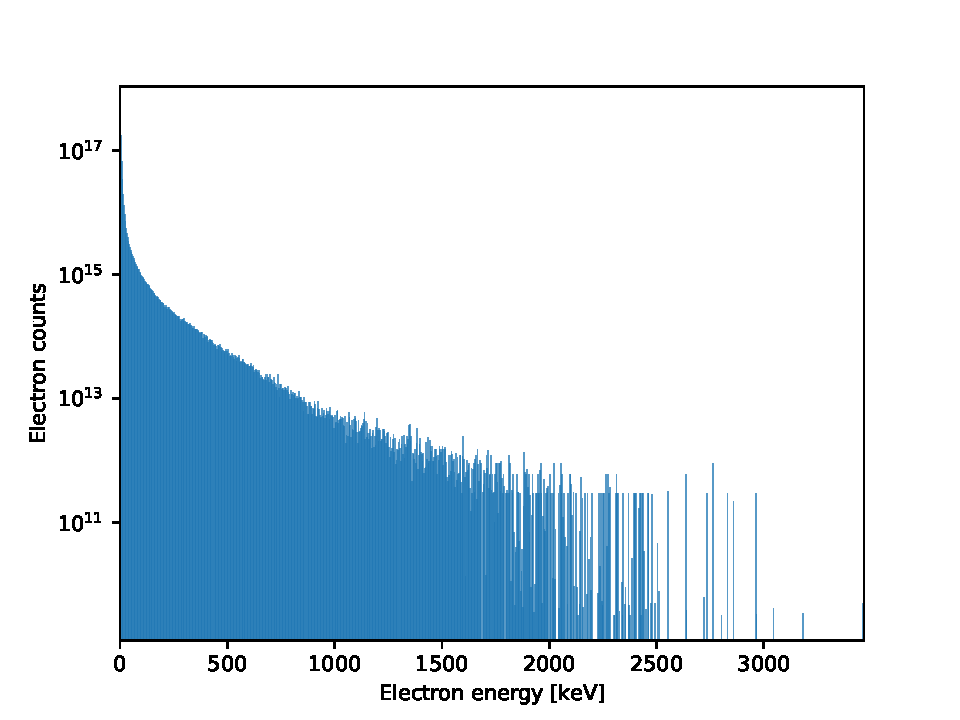
\includegraphics[width=0.9\textwidth]{figures/example-histogram}
	\caption{An example of electron energy distribution of 2D EPOCH simulation with intensity of laser $I=10^{19}\,\mathrm{W.cm}^{-2}$, characteristic scale of the exponential preplasma profile $L=0.1\,\mathrm{\mu m}$ and angle of incidence with respect to target normal direction $\alpha = 10$°.}
	\label{fig:example-histogram}
\end{figure}
One can easily create the histogram from electron energies and their counts. An example of such histogram can be seen in the figure \ref{fig:example-histogram}. There are several things that need to be discussed.

Firstly, it is important to note that the $y$-axis is presented on a logarithmic scale to enhance readability. The extensive range of electron energies necessitates the use of relativistic formula. However, around the energies $E_k \approx 1900 \, \mathrm{keV}$ and more, the histogram exhibits irregularities - specifically, there are empty bins and several bins contain identical electron counts. These anomalies are attributed to the resolution of the simulation. Consequently, this portion of the spectrum is rendered questionable. This issue will be further addressed in the section dedicated to temperature fitting.

Last but not least, note the apparent exponential relationship between $N_i$ and $E_k$ in the energy spectrum between $E_k \approx 500 \, \mathrm{keV}$ and $E_k \approx 1500 \, \mathrm{keV}$:
\begin{equation}
	\label{eq:exp-distr}
	N_i = N_0 \cdot \mathrm{exp}\left( -\frac{E_i}{T}\right)\mathrm{,}
\end{equation}
where $N_i$ is count in $i$-th bin and $E_i$ is the corresponding energy and $T$ is temperature in units discussed in section \ref{sec:temperature-intro}. After the logarithmic transformation, the relationship is, of course, linear. The equation of \ref{eq:exp-distr} resembles exponential distribution with $1/T$ missing on the right-hand side. It is also not normalized, because it represents counts that have to add up to total number of electrons with that temperature. For the purpose of this thesis, we will call it the \textit{Boltzmann distribution}, even though it is not completely accurate.

Fitting the correct part of the histogram using equation \ref{eq:exp-distr} and estimating $T$ and $N_0$ is the first bigger part of this thesis. There are several obstacles, all of which are discussed in following sections.

\section{Boltzmann vs. Maxwellian distribution}
First of all, in section \ref{sec:temperature-intro}, where we introduced temperature as a quantity describing plasma, we said that the distribution of energies is usually considered to be Maxwellian. The question, whether we can fit our histogram using Boltzmann distribution, is therefore valid and needs to be addressed.

The equations for the Maxwellian $f_\mathrm{M}(E)$ and Boltzmann $f_\mathrm{B}(E)$ distributions can be after few simplifications regarding units defined as:
\begin{equation}
	f_\mathrm{M}(E)\mathrm{d}E = \frac{\sqrt{E}}{(T)^{3/2}}\exp\left(-\frac{E}{T}\right)\mathrm{d}E
\end{equation}
and
\begin{equation}
	f_\mathrm{B}(E)\mathrm{d}E = \frac{1}{T}\exp\left(-\frac{E}{T}\right)\mathrm{d}E.
\end{equation}
Ignoring that both are defined by the differential and taking logarithm of both $f_\mathrm{M}(E)$ and $f_\mathrm{B}(E)$ we get:
\begin{equation}
	\bar{f_\mathrm{M}}(E) = \ln\left(f_\mathrm{M}(E)\right) = \ln\left(\frac{\sqrt{E}}{(T)^{3/2}}\right)+\left(-\frac{E}{T}\right)
\end{equation}
and
\begin{equation}
	\bar{f_\mathrm{B}}(E) = \ln\left(f_\mathrm{B}(E)\right) = \ln\left(\frac{1}{T}\right)+\left(-\frac{E}{T}\right).
\end{equation}
These two equations describe the the distributions in a logarithmic scale. The first derivatives are then:
\begin{equation}
	\label{eq:slope-maxwell-log}
	\frac{\mathrm{d}\bar{f_\mathrm{M}}}{dE} =-\frac{1}{2}\frac{T^{3/2}}{\sqrt{E}}\frac{1}{T^{3/2}\sqrt{E}}-\frac{1}{T} = -\frac{1}{2E}-\frac{1}{T}
\end{equation}
and
\begin{equation}
	\label{eq:slope-boltzmann-log}
	\frac{\bar{f_\mathrm{B}}}{dE} = -\frac{1}{T}.
\end{equation}
The equations \ref{eq:slope-maxwell-log} and \ref{eq:slope-boltzmann-log} suggest that, in the logarithmic scale, the slopes of these distributions differ by $-\frac{1}{2E}$, which decreases with increasing $E$. In other words, the fit of $T$ can be replaced by fitting slope $s = -1/T$ of the histogram after logarithmic transformation. For large energies, the slopes of both discussed distributions are approximately equal. 

Moreover, the assumption of Boltzmann distribution allows us to fit not only the temperature, but also $N_0$, which is the total number of electrons in that distribution of hot electrons. If we keep the form of the distribution as in equation \ref{eq:exp-distr}, the total energy absorbed by the group of hot electrons $E_{\mathrm{tothot}}$ with temperature $T_\mathrm{hot}$ can be calculated as:
\begin{equation}
	E_{\mathrm{tothot}} = N_0\cdot T_\mathrm{hot}.
\end{equation}


\section{Exponential-sum fitting}
\label{sec:exp-fit}
Exponential-sum fitting has been a recognized challenge for many years. Forman S. Acton, a professor at Princeton University, addressed this issue in his 1970 book Numerical Methods That Work. Among various topics, he included an essay titled "What Not to Compute," wherein he described the fitting of sums of exponential functions as "extremely ill-conditioned"~\cite{acton1990}. Despite the inherent difficulty of this problem, this thesis endeavors to determine electron temperatures, necessitating the development of an effective solution to this challenging computational task. 

The task is to find the parameters $m, a_0, a_1,..., a_m, b_1,...b_m$ so that the function

\begin{equation}
	f(x) = a_0 + \sum_{i=1}^{m} a_i \mathrm{e}^{b_i x}
\end{equation}

generalizes the data as good as possible. Formally, for a set of data ($n$ data points) $\left(\left(x_1,y_1\right),..., \left(x_n,y_n\right)\right)$ we are minimizing error function

\begin{equation}
	e = \sum_{i=1}^{n}w_i(y_i-f(x_i))^2
\end{equation}

where $w_i$ are the weights.

Modern programming libraries provide access to well-known and generally efficient methods, such as non-linear least squares. However, due to the previously mentioned ill-conditioning, these methods do not yield satisfactory results in this context. The convergence of these methods is highly dependent on the quality of the initial guess, which poses a significant challenge. To date, significant efforts have been made to develop reliable methods for solving this problem. 

Notably, Prony's method \cite{prony1795} and its variations, as discussed in sources such as \cite{potts2010}, have been proposed. It was originally intended for signal approximation - specifically, the determination of complex parameters in exponential functions, similar to Fourier transformation.

Another, much simpler method is known as \textit{successive subtraction}~\cite{wiscombe1977}. This method is frequently employed for exponential decays (negative parameters $b_i$), which closely resemble our problem of exponential distributions. The core concept involves fitting the end of the decay with a single exponential function, subtracting this result from the data, and iteratively identifying all exponential components. The simplicity makes it a promising candidate for our problem, especially since our primary interest lies in determining the temperature of the hottest electrons -- the tail. However, automating this method can be challenging, as it is not straightforward how to select an interval that can be fitted as a tail in each iteration. Moreover, the tails of our histograms are not reliable as was discussed with regard of the example histogram in Figure \ref{fig:example-histogram}.

Another method worth considering is presented in \cite{wiscombe1977}. This method, called exponential sum fitting of transmissions (ESFT), was developed for fitting radiative transmission functions in the context of atmospheric research. ESFT too is an iterative method and might serve as an interesting alternative for future works.

We only mentioned a few methods. A summary with a deeper explanation of these and other methods can be found in \cite{wiscombe1977}, \cite{holmstrom2002} or in \cite{hokanson2013}.

If the goal is to fit only one of the exponentials, such as the parameters of the hot electrons distribution, the standard approach involves manually selecting the "correct" segment of the distribution and fitting it with a single exponential function. For instance, in \cite{cui2013}, where researchers study a problem similar to ours, they appear to use this technique to determine the temperature of hot electrons. The term "correct" is somewhat vague because it can be subjective and we do not have any metric that would quantify how well the segment was chosen. We can only work with the metrics describing the quality of fit itself.

The last mentioned option currently provides the most reliable approach to fitting the temperature of hot electrons. Even for hundreds of simulations, with the right tool, it is possible to fit manually every histogram within few hours. Having such dataset of histograms and temperatures is valuable for evaluating any method that is trying to automate the fitting process. A tool with an user interface was developed specifically for this purpose as a part of this work.

That being said, we still attempted to automate the fitting. We use and compare two different methods. 

In the first, we can estimate the the fit parameters of multi-exponential function using linearization trick. This step is explicit an non-iterative. The analytical explanation is presented in the following section.

The second method is more trivial. It is based on the assumption that the part of the spectrum where hot electrons dominate is \textit{reasonably} large. Compared to the first method, it much more resembles what is done when we do the fit manually -- search for region with the smallest slope which corresponds to the highest temperature. The trick here is to \textit{scan} through the histogram by fitting many smaller subsets after simple linearization. Then we choose as result the fit with the highest hot electron temperature estimate. We call this the \textit{Scanning} method and the detailed description of our implementation and the results will be found in Chapter \ref{ch:dataset}.

\subsection*{The 'Jacquelin' method}
\label{sec:jaquelin}
We will call the explicit estimation \textit{Jacquelin method}, because we will be referencing an article by J.Jacquelin who developed it for his own purpose \cite{jacquelin2014}. As we said, this method is explicit and non-iterative which is its main advantage. Note, that the original derivation presents a universal strategy for how to explicitly approximate any function that is a solution to some integral or differential equation. Let us start with derivation of the numerical algorithm for a function:
\begin{equation}
	\label{eq:orig-eq}
	y(x) = a_0 + a_1\mathrm{e}^{b_1x} + a_2\mathrm{e}^{b_2x}
\end{equation}

We start by calculating these integrals:
\begin{flalign*}
	\;\;\;\;\;\;\;\;\;\;\;\; S(x) & = \int_{x_0}^{x}y(t) \mathrm{d}t \\
	& = \int_{x_0}^{x}a_0 + a_1\mathrm{e}^{b_1t} + a_2\mathrm{e}^{b_2t} \mathrm{d}t \\
	& = a_0(x-x_0) + \frac{a_1}{b_1}(\mathrm{e}^{b_1x}-\mathrm{e}^{b_1x_0}) +
	\frac{a_2}{b_2}(\mathrm{e}^{b_2x}-\mathrm{e}^{b_2x_0}) &
\end{flalign*}

\begin{flalign*}
	\;\;\;\;\;\;\;\;\;\;\;\; SS(x) & = \int_{x_0}^x S(t)\mathrm{d}t \\
	& = \int_{x_0}^x\int_{x_0}^{t}y(u) \mathrm{d}u\mathrm{d}t \\
	& = \int_{x_0}^{x}a_0t + \frac{a_1}{b_1}\mathrm{e}^{b_1t} +
	\frac{a_2}{b_2}\mathrm{e}^{b_2t} - \left(\frac{a_1}{b_1}\mathrm{e}^{a_1 x_0}+\frac{a_2}{b_2}\mathrm{e}^{a_2 x_0}+a_0x_0\right)\mathrm{d}t \\
	& = \frac{1}{2}a_0x^2 - \left(\frac{a_1}{b_1}\mathrm{e}^{a_1 x_0}+\frac{a_2}{b_2}\mathrm{e}^{a_2 x_0}+a_0x_0\right)(x-x_0) -\frac{1}{2}a_0x_0^2 \\ 
	& \;\;\; + \frac{a_1}{b_1^2}\left(\mathrm{e}^{b_1x} - \mathrm{e}^{b_1x_0}\right)  + \frac{a_2}{b_2^2}\left(\mathrm{e}^{b_2x} - \mathrm{e}^{b_2x_0}\right) &&
\end{flalign*}

Now, if we reorganize the terms it can be shown that there are constants $A$, $B$, $C$, $D$ and $E$ so that $y(x)$ can be written as:
\begin{equation}
	\label{eq:lin}
	y(x) = A\cdot SS(x)+B\cdot S(x) + C x^2 + Dx + E.
\end{equation}
By comparing coefficients in from of the exponential terms $\mathrm{e}^{b_1 x}$ and $\mathrm{e}^{b_2 x}$ we get:
\begin{align}
	a_1 & = A\frac{a_1}{b_1^2} + B\frac{a_1}{b_1}  \\
	a_2 & = A\frac{a_2}{b_2^2} + B\frac{a_2}{b_2}
\end{align}
From there, it is possible to see that both $b_1$ and $b_2$ are roots of the quadratic equation:
\begin{equation}
	\label{eq:quadratic}
	b^2 - bB - A = 0.
\end{equation}
$b_1$ and $b_2$ are then:
\begin{equation}
	\label{eq:roots}
	b_{1,2} = \frac{1}{2}\left(B \pm \sqrt{B^2 + 4A}\right)
\end{equation}

The equation \ref{eq:lin} is linear in the unknown parameters $A,..,E$ and after discretization it can be rewritten as: 
\begin{equation}
	\label{eq:lin-vec}
	\boldsymbol{y}=\boldsymbol{X}\cdot \boldsymbol{b}
\end{equation}
where $\boldsymbol{y}$ is vector:
\begin{equation}
	\boldsymbol{y} =
	\begin{pmatrix}
		y_1 \\
		y_2 \\
		\vdots \\
		y_n  
	\end{pmatrix}
\end{equation} 	

Denoting $S_k=S(x_k)$ and $SS_k=SS(x_k)$ we can write:
\begin{equation}
	\boldsymbol{X} =
	\begin{pmatrix}
		SS_1 & S_1 & x_1^2 & x_1 & 1 \\
		SS_2 & S_2 & x_2^2 & x_2 & 1 \\
		SS_3 & S_3 & x_3^2 & x_3 & 1 \\
		\vdots & \vdots & \vdots & \vdots & \vdots \\
		SS_n & S_n & x_n^2 & x_n & 1  
	\end{pmatrix}
\end{equation}
and 
\begin{equation}
	\boldsymbol{b} =
	\begin{pmatrix}
		A \\
		B \\
		C \\
		D \\
		E  
	\end{pmatrix}.
\end{equation}

We can use the well-known least squares method to calculate the parameters $A,...,E$. We sort the data so that if $i<j$, then $x_i<x_j$ for $\forall i,j \in \{1,..,n\}$. The integrals are computed numerically as:
\begin{equation}
	S_i = \left\{
	\begin{array}{ll}
		0 & i=0 \\
		S_{i-1} + \frac{1}{2}(y_i+y_{i-1})(x_i-x_{i-1}) & i\in\{2,...n\}
	\end{array}
	\right.
\end{equation}
and
\begin{equation}
	SS_i = \left\{
	\begin{array}{ll}
		0 & i=0 \\
		SS_{i-1} + \frac{1}{2}(S_i+S_{i-1})(x_i-x_{i-1}) & i\in\{2,...n\}
	\end{array}
	\right.
\end{equation}

Now, the solution to the linear equation \ref{eq:lin-vec} can be written as:
\begin{equation}
	\boldsymbol{b}=\left(\boldsymbol{X}^T\boldsymbol{X}\right)^{-1}\cdot (\boldsymbol{X}^T\boldsymbol{y})
\end{equation}
which in our case can be expanded to:
\begin{equation}
	\label{eq:lin-reg}
	\begin{pmatrix}
		A \\
		B \\
		C \\
		D \\
		E  
	\end{pmatrix} 
	=
	\begin{pmatrix}
		\sum\limits_{i=1}^nSS_i^2 & \sum\limits_{i=1}^nSS_iS_i & \sum\limits_{i=1}^nSS_ix_i^2 & \sum\limits_{i=1}^nSS_ix_i & \sum\limits_{i=1}^nSS_i \\
		\sum\limits_{i=1}^nSS_iS_i & \sum\limits_{i=1}^nS_i^2 & \sum\limits_{i=1}^nS_ix_i^2 & \sum\limits_{i=1}^nS_ix_i & \sum\limits_{i=1}^nS_i \\
		\sum\limits_{i=1}^nSS_ix_i^2 & \sum\limits_{i=1}^nS_ix_i^2 & \sum\limits_{i=1}^nx_i^4 & \sum\limits_{i=1}^nx_i^3 & \sum\limits_{i=1}^nx_i^2 \\
		\sum\limits_{i=1}^nSS_ix_i & \sum\limits_{i=1}^nS_ix_i & \sum\limits_{i=1}^nx_i^3 & \sum\limits_{i=1}^nx_i^2 & \sum\limits_{i=1}^nx_i \\
		\sum\limits_{i=1}^nSS_i & \sum\limits_{i=1}^nS_i & \sum\limits_{i=1}^nx_i^2 & \sum\limits_{i=1}^nx_i & n  
	\end{pmatrix}^{-1}
	\begin{pmatrix}
		\sum\limits_{i=1}^nSS_iy_i \\
		\sum\limits_{i=1}^nS_iy_i \\
		\sum\limits_{i=1}^nx_i^2y_i \\
		\sum\limits_{i=1}^nx_iy_i \\
		\sum\limits_{i=1}^ny_i  
	\end{pmatrix}
\end{equation}

After we compute $b_1$ and $b_2$ from $\boldsymbol{b}$, we still have 3 unknown parameters $a_0$, $a_1$ and $a_2$. For those, we will take the original equation \ref{eq:orig-eq}. As it is already linear in the parameters $a_0$, $a_1$ and $a_2$, we only need to pre-compute the values of $\alpha_k=\mathrm{e}^{b_1x_k}$ and $\beta_k =\mathrm{e}^{b_2x_k}$.
One can see that we get a very similar equation as \ref{eq:lin-reg}, that can be written in this form:
\begin{equation}
	\begin{pmatrix}
		a_0 \\
		a_1 \\
		a_2
	\end{pmatrix} 
	=
	\begin{pmatrix}
		n & \sum\limits_{i=1}^n\alpha_i & \sum\limits_{i=1}^n\beta_i  \\
		\sum\limits_{i=1}^n\alpha_i & \sum\limits_{i=1}^n\alpha_i^2 & \sum\limits_{i=1}^n\alpha_i\beta_i  \\
		\sum\limits_{i=1}^n\beta_i & \sum\limits_{i=1}^n\alpha_i\beta_i & \sum\limits_{i=1}^n\beta_i^2
	\end{pmatrix}^{-1}
	\begin{pmatrix}
		\sum\limits_{i=1}^ny_i \\
		\sum\limits_{i=1}^n\alpha_iy_i \\
		\sum\limits_{i=1}^n\beta_iy_i
	\end{pmatrix}
\end{equation}

In \cite{jacquelin2014}, only the case without the constant $a_0$ is presented, but as we have shown the derivation of the generalized version with constant is not difficult. An extension of Jacquelin method for more than two exponential terms is also not very complicated. Note that adding one term adds two parameters, which leads to matrix of size $7\times7$. However, it always leads to solving for the roots of the polynomial created by the first $N$ elements of the vector $\boldsymbol{b}$, where $N$ is the number of exponential terms. In case of two exponential terms, equation \ref{eq:roots} solves for the roots of the polynomial of Equation \ref{eq:quadratic}. In case of three exponential terms, we would need to calculate $SSS(x)$ from $SS(x)$. There would also be a term $x^3$. If we set $\boldsymbol{X}$ as $\left[SSS(x),SS(x),S(x),x^3,x^2,x^1,1\right]$, we would solve for the roots of:
\begin{equation}
	b^3-Cb^2-Bb-A=0.
\end{equation}

It is necessary to note, that this algorithm is prone to numerical defects coming from the fact that there is a cumulative error related to the calculation of the partial sums. For that reason the resulting matrices can be singular or the polynomial can have imaginary roots. Such scenario does not produce reasonable result.

In \cite{mokhomo2021}, Mokhomo et al. did numerical experiments where they have shown that similar method (derived from differential instead of integral equations) can be used for fitting, but does not yield precise estimation results even for noiseless data. Nevertheless, it is an explicit algorithm for approximation of parameters which then can be used as initial guess for more advanced techniques.

When it comes to uncertainty of the coefficients, there are two possibilities. First, it is possible to propagate the experimental error from $y_i$ all the way to the final coefficients. The derivation can be found in \cite{lecca2021}. However, we do not have the standard error of the histogram bins. In principle, this can be obtained by repeating the simulation with the same input parameters but with a different seed for the random number generator which provides initial velocities for particles based on Maxwellian distribution. 

The second option is to take the formula for linear regression and calculate the error estimation directly from that from that. In that case, we calculate estimates $\Delta A$ and $\Delta B$ as standard deviations for $A$ and $B$. Then, using the error propagation formula for the quadratic roots we get:
\begin{equation}
	\label{eq:b-coef-error1}
	\Delta b_{1,2} = \sqrt{\frac{\Delta A^2}{(B^2 + 4A)} + \frac{\Delta B^2}{4} \left(1 \pm \frac{B}{\sqrt{B^2 + 4A}}\right)^2}
\end{equation}
where $\Delta b_1$ and $\Delta b_2$ are the estimates of standard deviations for $b_1$ and $b_2$.
The standard deviations of $a_0$, $a_1$ and $a_2$ are calculated directly from the second linear regression.

We will not follow the same approach of error estimation for more exponential terms, but theoretically, it could be done. In Chapter \ref{ch:dataset}, we will talk about how this method works on our data.

